\documentclass{article}

\usepackage[compat=1.1.0]{tikz-feynhand}

\tikzexternalize[prefix=graphics/]

\tikzset{external/force remake}

\begin{document}

\tikzsetnextfilename{part-2g2a-t1}
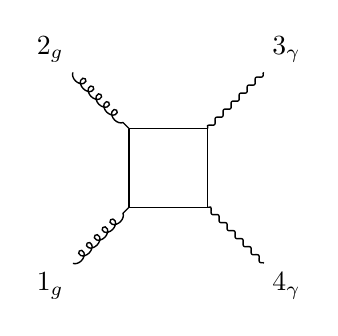
\begin{tikzpicture}
    \begin{feynhand}

        \vertex (o0) at (-1.5,-1.5) {$1_g$};
        \vertex (o1) at (-1.5,1.5) {$2_g$};
        \vertex (o2) at (1.5,1.5) {$3_\gamma$};
        \vertex (o3) at (1.5,-1.5) {$4_\gamma$};

        \vertex (i0) at (-0.5,-0.5);
        \vertex (i1) at (-0.5,0.5);
        \vertex (i2) at (0.5,0.5);
        \vertex (i3) at (0.5,-0.5);

        \propag [gluon] (o0) to (i0);
        \propag [gluon] (o1) to (i1);
        \propag [photon] (o2) to (i2);
        \propag [photon] (o3) to (i3);

        \propag [plain] (i0) to (i1);
        \propag [plain] (i1) to (i2);
        \propag [plain] (i2) to (i3);
        \propag [plain] (i3) to (i0);

    \end{feynhand}
\end{tikzpicture}

\tikzsetnextfilename{part-2g2a-t2}
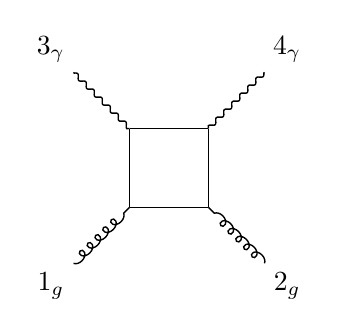
\begin{tikzpicture}
    \begin{feynhand}

        \vertex (o0) at (-1.5,-1.5) {$1_g$};
        \vertex (o1) at (-1.5,1.5) {$3_\gamma$};
        \vertex (o2) at (1.5,1.5) {$4_\gamma$};
        \vertex (o3) at (1.5,-1.5) {$2_g$};

        \vertex (i0) at (-0.5,-0.5);
        \vertex (i1) at (-0.5,0.5);
        \vertex (i2) at (0.5,0.5);
        \vertex (i3) at (0.5,-0.5);

        \propag [gluon] (o0) to (i0);
        \propag [photon] (o1) to (i1);
        \propag [photon] (o2) to (i2);
        \propag [gluon] (o3) to (i3);

        \propag [plain] (i0) to (i1);
        \propag [plain] (i1) to (i2);
        \propag [plain] (i2) to (i3);
        \propag [plain] (i3) to (i0);

    \end{feynhand}
\end{tikzpicture}

\tikzsetnextfilename{part-2g2a-t3}
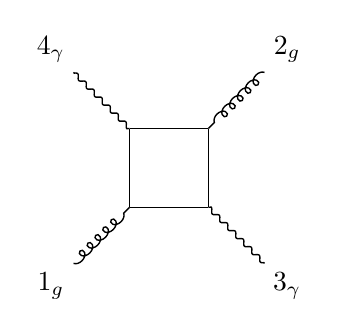
\begin{tikzpicture}
    \begin{feynhand}

        \vertex (o0) at (-1.5,-1.5) {$1_g$};
        \vertex (o1) at (-1.5,1.5) {$4_\gamma$};
        \vertex (o2) at (1.5,1.5) {$2_g$};
        \vertex (o3) at (1.5,-1.5) {$3_\gamma$};

        \vertex (i0) at (-0.5,-0.5);
        \vertex (i1) at (-0.5,0.5);
        \vertex (i2) at (0.5,0.5);
        \vertex (i3) at (0.5,-0.5);

        \propag [gluon] (o0) to (i0);
        \propag [photon] (o1) to (i1);
        \propag [gluon] (o2) to (i2);
        \propag [photon] (o3) to (i3);

        \propag [plain] (i0) to (i1);
        \propag [plain] (i1) to (i2);
        \propag [plain] (i2) to (i3);
        \propag [plain] (i3) to (i0);

    \end{feynhand}
\end{tikzpicture}

\end{document}
